\documentclass[11pt]{article}
\usepackage{graphicx}

\begin{document}
\section{Autotransformadores}
Los autotransformadores poseen una parte del devanado en común, que corresponde tanto al 
primario como al secundario. 
El principio de funcionamiento es el mismo que el del transformador común, entonces la relación de 
transformación entre las tensiones, las intensidades de corriente y el número de vueltas se mantienen.

Las corrientes primarias y secundarias están en oposición y la corriente total que circula por las espiras
en común es igual a la diferencia de la corriente del devanado de baja tensión y el devanado de alta tensión
\begin{equation}
    I_c = I_{AT} - I_{BT} \quad \textnormal{si } V_{AT} > V_{BT}   
\end{equation}
Para que un autotransformador funcione adecuadamente, los devanados deben tener el mismo sentido de bobinado.

\subsection{Autotransformadores Reductores}
Si se aplica una tensión alterna entre los puntos A y B, y se mide la tensión de salida entre los puntos C y D,
se dice que el autotransformador es un reductor de tensión

\begin{figure}[h]
    \begin{center}
        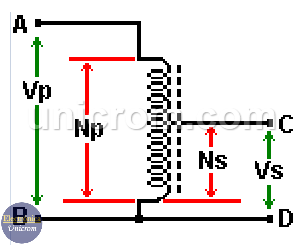
\includegraphics[width=200px]{autotransformador-reductor.png}
    \end{center}
    \caption{Autotransformador reductor}
\end{figure}

En este caso, la relación de vueltas del autotransformador es:
\begin{equation}
    \frac{N_s}{N_p} < 1 
\end{equation}

\end{document}